\chapter{Development Methodolgy}

\textcolor{red}{\textbf{TODO: Possibly restructure this, it\'s a start for now. Not 100\% sure what Neil\'s looking for here.}}

\section{Initial Project Plan}

Upon starting the project, we met as a group and decided on a standard style of development which would work best between all of us. After some discussion, we concluded that a \textit{Scrumban}\cite{scrumban} style of development would best fit our needs. Due to the relatively short duration of the project, and our team consisting of only eight developers, we decided on adopting this rather hands off development approach which focuses on flexibility and being able to change and adapt the project plan and sprints as the project progresses. The \textit{Scrumban} methodology was also suited to the project as the two technologies we were required to use, Java EE and .NET Core, were new to all of the members of our team, making estimating sprints and velocity quite difficult. 

We began the project by breaking the project specification down into disitinct microservices, and deciding which technologies would be best suited to each service. \textbf{TODO: Link to figure below}

\begin{figure}[H]
    \centering
    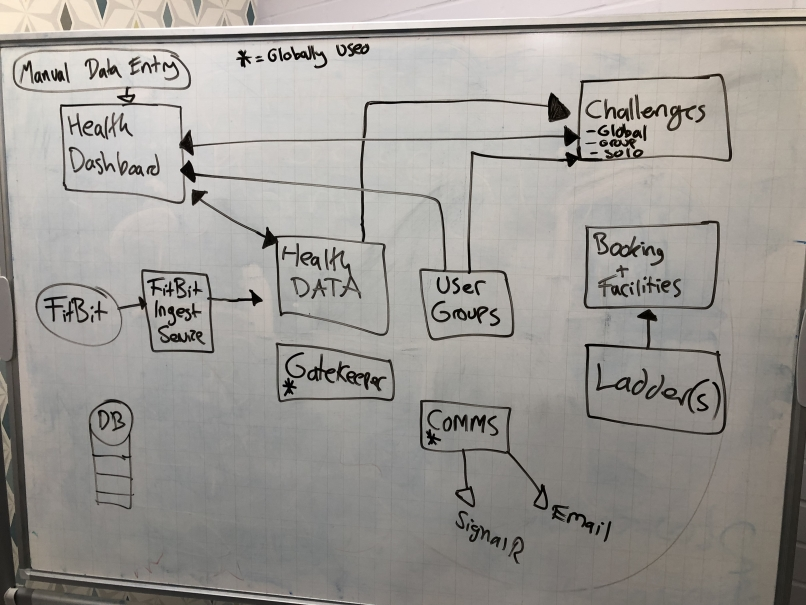
\includegraphics[width=\textwidth]{Images/Initial_Spec_Chart.jpg}
    \caption{An initial design diagram which was used to help break down the project into smaller microservices and gain a rough understanding how each microservice could interact}
\end{figure}

Once the individual microservices had been decided upon, we set out on allocating each microservice to two members of the team and assinging each service a priority ranking between 1 and 3, depending on how the services depended on one another. Services marked with a priority of 1 were core parts of the \textit{AberFitness} infrastructure on which many other parts of the system relied on their APIs in order to function correctly, such as the \textit{Health Data Repository} microservice.  \textbf{TODO: Link to figure below}

\begin{figure}[H]
    \centering
    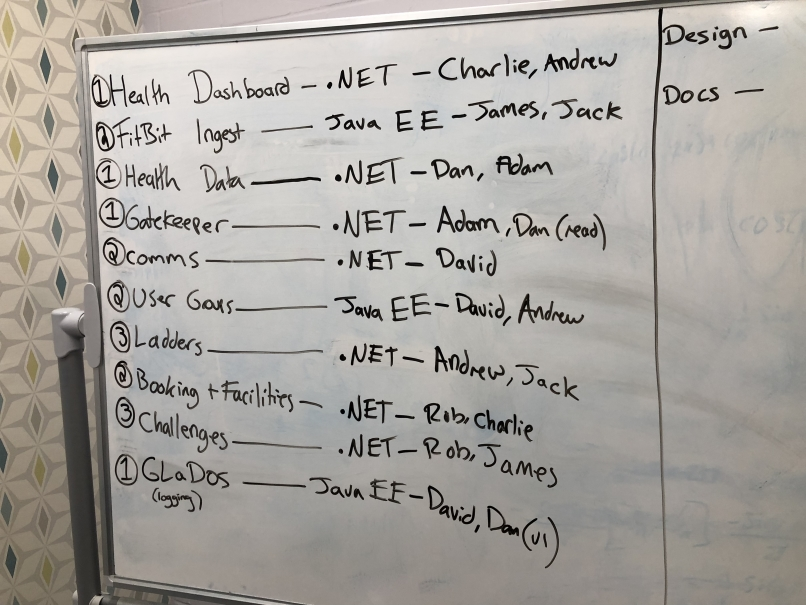
\includegraphics[width=\textwidth]{Images/Numbering_Microservices.jpg}
    \caption{Initial plan for ordering microservices in terms of priority and allocating them to members of the team for development}
\end{figure}


\section{Supporting Tools}
\subsection{GitHub \& TravisCI}
Each microservice for \textit{Aber Fitness} was hosted on \textit{GitHub}\footnote{https://github.com/sem5640-2018}. \textit{GitHub} provided many features which proved incredibly useful during the development phase, such as tight integration with \textit{Slack} for notifications straight to our chatrooms and integration with \textit{TravisCI} to automatically trigger unit tests and \textit{Docker} image builds. We also developed a development pattern of requiring all code to be peer reviewed through the use of pull requests and branch protection, a collection of settings which require that a series of conditions have been met before a pull request is able to be merged into the \textit{development} or \textit{master} branch. We configured branch protection in order to ensure that only tested, peer reviewed code would be committed into any upstream branch to reduce the likelihood of errors being introduced into the system and so that any issues could be caught early on. 

\begin{figure}[H]
    \centering
    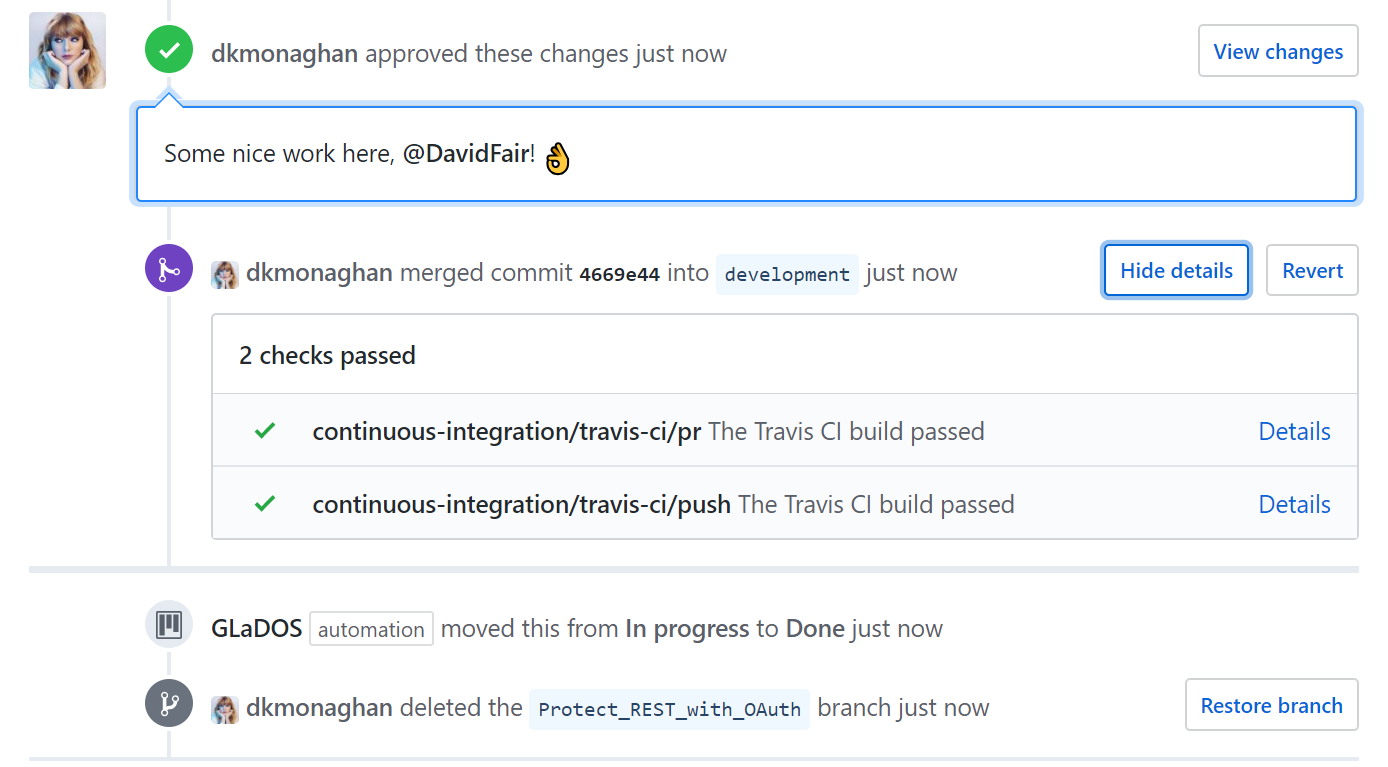
\includegraphics[width=\textwidth]{Images/approve_pr.png}
    \caption{A screenshot from \textit{GitHub} showing a pull request on the \textit{GLaDOS} repository being peer reviewed and also checks from \textit{TravisCI} passing before being merged into an upstream branch.}
\end{figure}

Once a pull request had been approved and merged, \textit{TravisCI} would then be responsible for building and pushing the \textit{Docker} image to \textit{Docker Hub}.

\begin{figure}[H]
    \centering
    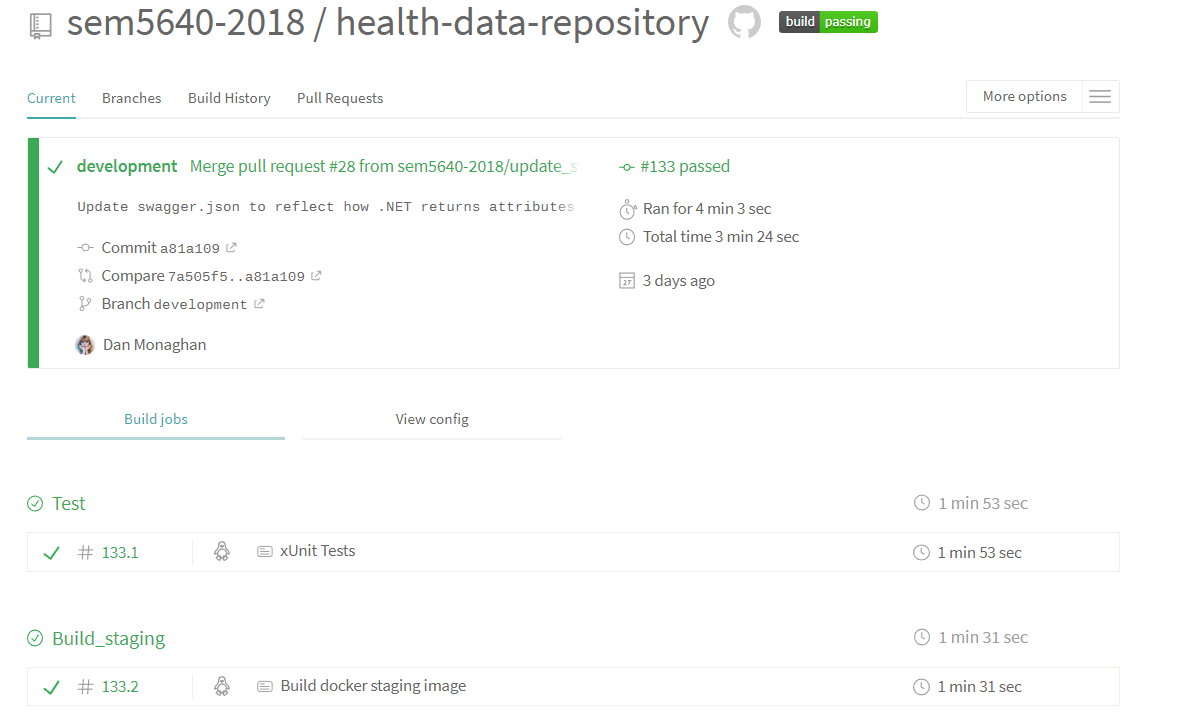
\includegraphics[width=\textwidth]{Images/travis_builds_overview.png}
    \caption{A screenshot from \textit{TravisCI} demonstrating a pull request being merged into the \textit{development} branch, re-passing unit tests once merged and then building the \textit{Docker} image}
\end{figure}

\subsection{Swagger}
\begin{figure}[H]
    \centering
    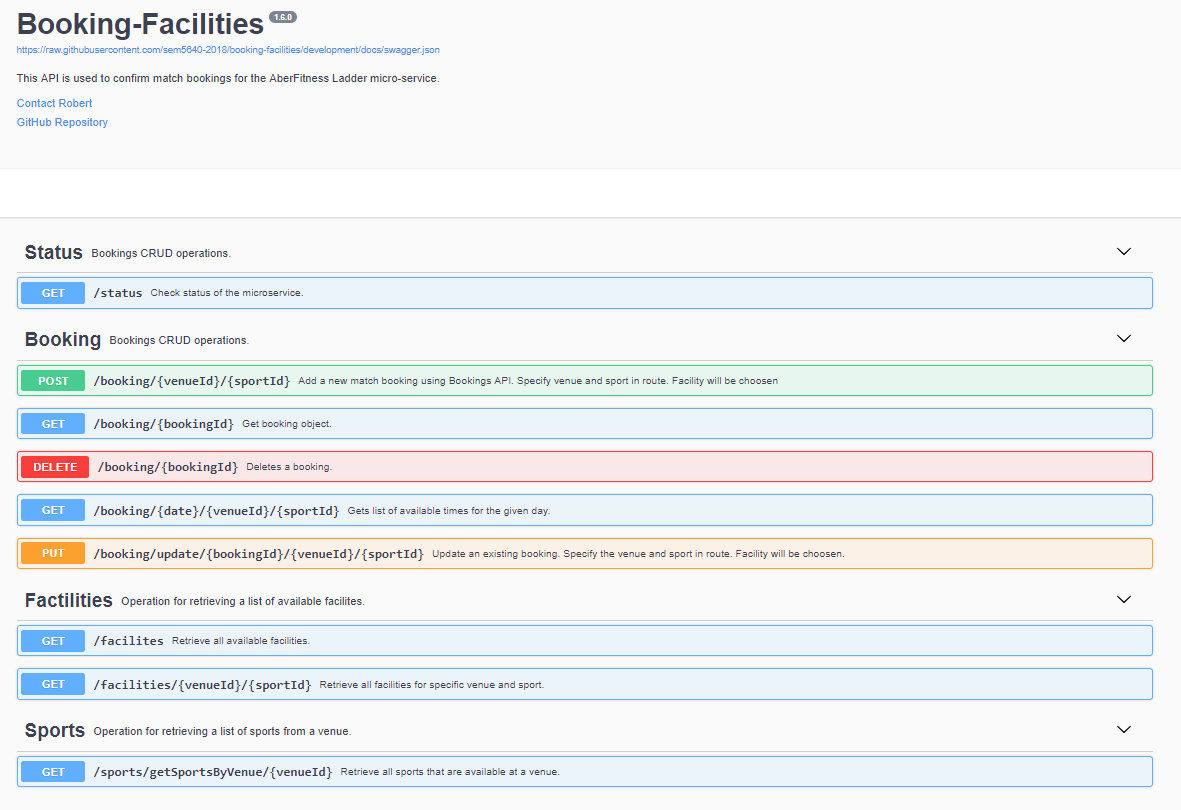
\includegraphics[width=\textwidth]{Images/Swagger.png}
    \caption{The Swagger interface for the \textit{Booking Facilities} microservice}
\end{figure}

\textit{Swagger} is a web based application for viewing API specifications. Each microservice within \textit{Aber Fitness} has a file located at \lstinline{docs/swagger.json} which defines its API endpoints and any associated data models. \textit{Swagger} was a crucial part of the development process as it allowed us to draft up API specifications prior to development in order to get feedback from other members of the group, and allowed issues to be identified early on in the event that a draft API specification lacked endpoints which would be required by other microservices. 


\subsection{Portainer}
\begin{figure}[H]
    \centering
    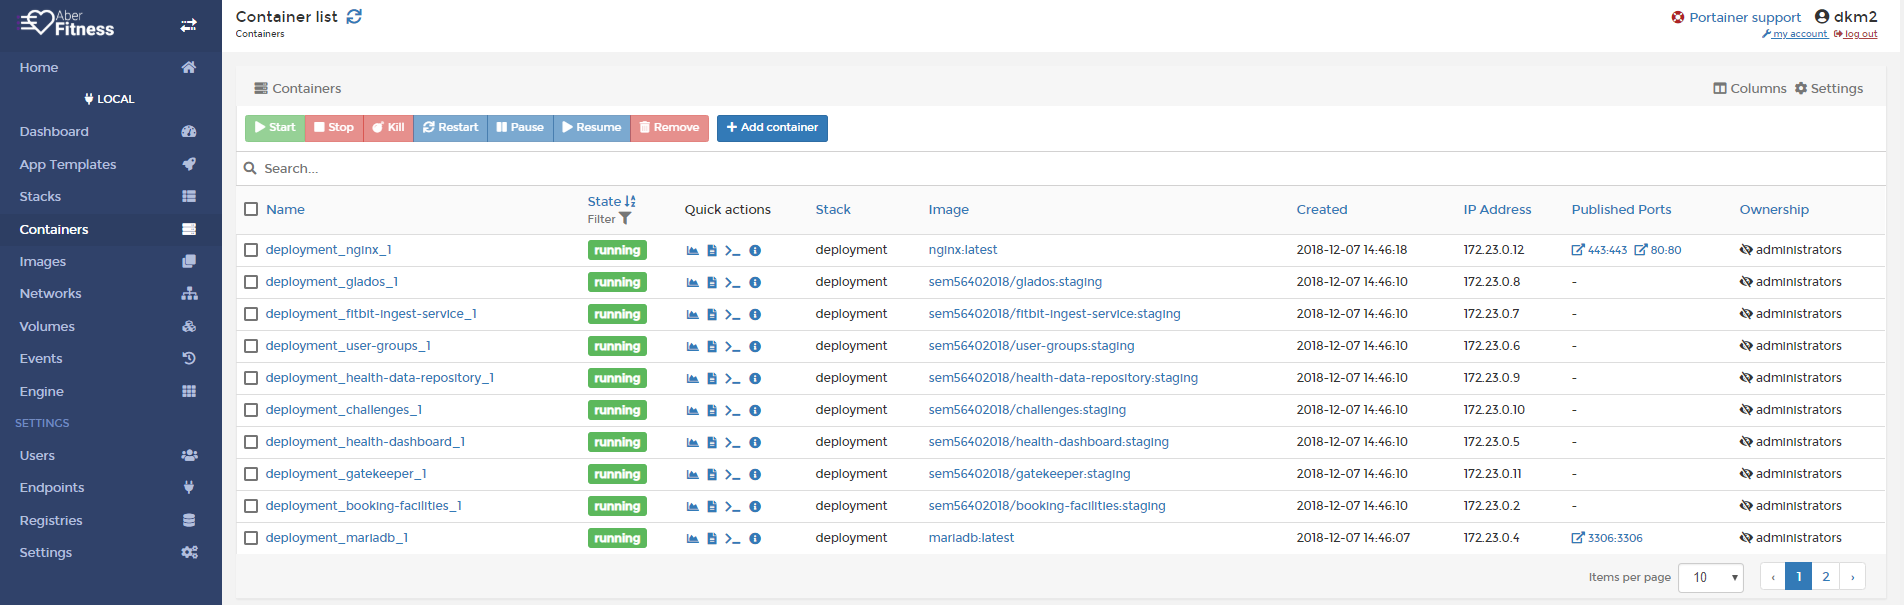
\includegraphics[width=\textwidth]{Images/Portainer.png}
    \caption{The Portainer interface for our staging / development Docker host, \lstinline{docker2-m56.dcs.aber.ac.uk}}
\end{figure}

\textit{Portainer} provides a dashboard for managing volumes, networks, images and containers on \textit{Docker} hosts. Throughout the initial configuration of the \textit{Docker} images, \textit{Portainer} proved invaluable as it provided the ability to quickly and easily understand what the host was running. \textbf{TODO: More here probably.}

\subsection{Docker Hub}
\textit{Docker Hub} is a platform provided by \textit{Docker} which allows \textit{Docker} container images to be uploaded and hosted, and easily pulled down by the \lstinline{docker-compose} script. As part of our build process (\textbf{TODO: reference build pipline diagram here}), images are built by \textit{TravisCI} and then pushed to \textit{Docker Hub} before being pulled down onto the \textit{Docker} hosts.


\subsection{Slack \& Deployment}
\textit{Slack} is an online text based chat service designed for offices and teams, and paticuarly suits itself to the development of software. The group used \textit{Slack} extensively throughout the development of \textit{Aber Fitness} not only to communicate and discuss progress, ideas and troubleshoot problems, but also made extensive use of \textit{Slack}'s integrations with services such as \textit{TravisCI} and \textit{GitHub}. 

\begin{figure}[H]
    \centering
    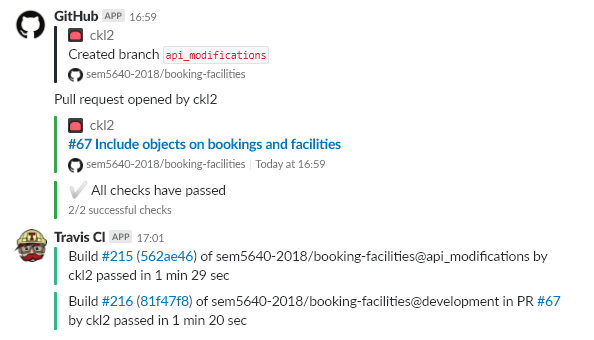
\includegraphics[width=\textwidth]{Images/Slack_Travis_GitHub.png}
    \caption{A screenshot of the \textit{Slack} channel \lstinline{\#dev-booking-facilities} demonstrating the integrations between \textit{Slack}, \textit{GitHub} and \textit{TravisCI}}
\end{figure}

\textit{Slack} also played a major role in our deployment strategy when rolling out updated \textit{Docker} images to our staging host. Due to the nature of the configuration of the two \textit{Docker} hosts we had been provided by the Computer Science department we ran into many issues with our deployment process, primarily to do with permissions on the host. Each member of the team had their own individual log in to the hosts, however we would frequently run into permissions errors when performing commands like \lstinline{git pull}. Other issues we had involved team members forgetting the specific set of commands which needed to be executed, wasting valuable development time. \textbf{TODO: figure no.}

\begin{figure}[H]
    \centering
    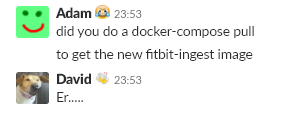
\includegraphics[width=0.5\textwidth]{Images/aberfitness_slack_bot_reason_why.png}
    \caption{An example situation where the execution of \lstinline{docker-compose pull} caused a large amount of confusion amongst \textit{Aber Fitness} developers}
\end{figure}


\textit{Slack} ended up providing us with an elegant solution to this through its ability to easily call a webhook when a user typed a specific message in a chat channel. A quick \textit{Slack} application was put together to automatically pull the latest \lstinline{docker-compose.yml} file from GitHub, as well as updating all the \textit{Docker Hub} images, then re-deploying the stack. This could all be done from within \textit{Slack} itself through the \lstinline{/deploy} command. \textbf{TODO: Figure no.}

\begin{figure}[H]
    \centering
    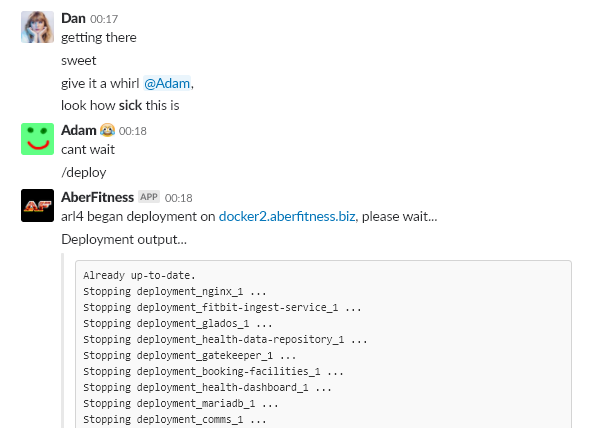
\includegraphics[width=0.9\textwidth]{Images/aberfitness_slack_bot.png}
    \caption{A demonstration of the \lstinline{/deploy} command being used to re-deploy \textit{Aber Fitness} onto the staging host}
\end{figure}

